\vspace*{1em}

Recall from Problem \ref{problem 4.8} that given two multiplicative functions $f,g:\zz_+ \to \cc$, the function, that we called \emph{convolution}, $(f*g):\zz_+ \to \cc$, defined as
\[(f*g)(n) \coloneqq \sum_{d \in \mathscr{D}(n)}f(d)g\left(\frac{n}{d}\right),\]
is also multiplicative.\\
\\
Take $f = \mu$, the M{\"o}bius function (see Problem \ref{problem 4.7}) and $g = \id$, i.e., $g(n) = n$ for all positive integers $n$. Then, 
\begin{align*}
(\mu * \id)(p^e) &= \sum_{d \in \mathscr{D}(p^e)}\mu(d)\id\left(\frac{n}{d}\right)\\[0.5em]
&= \sum_{k =0}^e \mu(p^k)\left(\frac{p^e}{p^k}\right)\\[0.5em]
&= \mu(1)p^e + \mu(p)p^{e-1} + \sum_{k =2}^e \mu(p^k)\left(\frac{p^e}{p^k}\right)\\[0.5em]
&= p^e - p^{e-1},\quad\text{since $\mu(p^k) = 0$, for $k\geq 2$}\\[0.5em]
&= p^{e-1}(p - 1)\\[0.5em]
&= \varphi(p^e)
\end{align*}
Hence, by multiplicativity of $\mu * \id$ and $\varphi$, we conclude that $\mu*\id = \varphi$

\vspace*{1em}

\begin{lemma}\label{totientsum}
Let $n$ be a positive integer, then we have
\[\sum_{d\in \mathscr{D}(n)}\varphi(d) = n\]
\end{lemma}
\begin{proof}
We have $\varphi = \mu * \id = \id * \mu$, by computations above and Problem \ref{Problem 12.1}. From Problem \ref{problem 4.7} we know that
\begin{align*}\label{mobiussum}
\sum_{d\in \mathscr{D}(n)}\mu(d) = \begin{cases} 1 & n=1\\[0.2em] 0 & n>1\end{cases}\tag{$\bigstar$}
\end{align*}
Let $\one:\zz_+ \to \cc$ be the constant function that's identically $1$, i.e., $\one(n) = 1$ for every $n$. Then \refp{mobiussum} can be rewritten as follows
\[(\mu*\one)(n) = \sum_{d\in \mathscr{D}(n)}\mu(d)\,\one\!\left(\frac{n}{d}\right) = \sum_{d\in \mathscr{D}(n)}\mu(d)\cdot 1 = \sum_{d\in \mathscr{D}(n)}\mu(d) = \begin{cases} 1 & n=1\\[0.2em] 0 & n>1\end{cases}\]
%\begin{align*}
%(\mu*\one)(n) &= \sum_{d\in \mathscr{D}(n)}\mu(d)\,\one\!\left(\frac{n}{d}\right)\\[0.5em]
%&= \sum_{d\in \mathscr{D}(n)}\mu(d)\cdot 1\\[0.5em]
%&= \sum_{d\in \mathscr{D}(n)}\mu(d)\\[0.5em]
%&= \begin{cases} 1 & n=1\\[0.2em] 0 & n>1\end{cases}
%\end{align*}
Note that this tells us that $\mu * \id = \epsilon$, where $\epsilon$ is as defined in Problem \ref{Problem 12.1}. Similarly, 
\[\sum_{d\in \mathscr{D}(n)}\varphi(d) = (\varphi*\one)(n)\]
Now, again by Problem \ref{Problem 12.1}, we get 
\begin{align*}
\varphi*\one &= (\id * \mu) * \one\\[0.5em]
&= \id * (\mu * \one)\\[0.5em]
&= \id *\ \epsilon\\[0.5em]
&= \id
\end{align*}
Therefore, $\displaystyle\sum_{d\in \mathscr{D}(n)}\varphi(d) = (\varphi*\one)(n) = \id(n) = n$.
\end{proof}

\vspace*{2em}

{\bf Primitive Roots and Polynomials.} Let $p$ be prime and $a \in \Phi(p)$ (equivalently, $p\nmid a$). We define $\ell(a)$ as the length of the cycles in the dynamics of \fbox{$\times a \modar{p}$} within $\Phi(p)$.\\
\\
We have seen, while proving Theorem \ref{euler-fermat} (Euler-Fermat), that $\ell(a) \mid \varphi(p) = p-1$.

\vspace*{1em}

\begin{definition}
Say $a$ is a primitive root modulo $p$ if $\ell(a) = p-1$. Equivalently, if there's only one cycle in the dynamics of \fbox{$\times a \modar{p}$} within $\Phi(p)$.
\end{definition}

%\vspace*{1em}

\emph{e.g.}\quad $p = 7$

\vspace*{1em}

\begin{minipage}{0.15\textwidth}
\qquad $a = 1$ 
\end{minipage}
\quad
\begin{minipage}{0.25\textwidth}
\[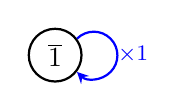
\begin{tikzpicture}[->,>=stealth,auto,node distance=3cm,
  thick,main node/.style={circle,draw}]

  \node[main node] (1) {$\overline{1}$};
\draw[blue]	(1.37) arc (135:-135:3mm) node[pos=0.3,below right] {\footnotesize$\times 1$} (1);
\end{tikzpicture}\]
\end{minipage}
\quad\!
\begin{minipage}{0.53\textwidth}
$\ell(1) = 1 \neq 7 - 1$, so $1$ is \emph{not} primitive. 
\end{minipage}

\vspace*{2em}

\begin{minipage}{0.15\textwidth}
\qquad $a = 2$ 
\end{minipage}
\begin{minipage}{0.25\textwidth}
\[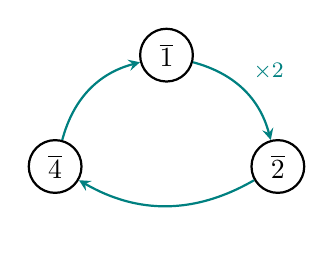
\begin{tikzpicture}[->,>=stealth,auto,node distance=2cm,
  thick,main node/.style={circle,draw}]

  \node[main node] (1) {$\overline{1}$};
  \node[main node] (2) [below right of= 1] {$\overline{2}$};
  \node[main node] (3) [below left of=1] {$\overline{4}$};
\path[every node/.style={font=\sffamily\small}]
	(1) edge[teal,bend left] node[] {\footnotesize$\times 2$} (2)
	(2) edge[teal,bend left] node[] {} (3)
	(3) edge[teal,bend left] node[] {} (1);
\end{tikzpicture}\]
\end{minipage}
\qquad
\begin{minipage}{0.53\textwidth}
$\ell(2) = 3 \neq 7 - 1$, so $2$ is \emph{not} primitive. 
\end{minipage}

\vspace*{2em}

\begin{minipage}{0.15\textwidth}
\qquad $a = 3$ 
\end{minipage}
\begin{minipage}{0.25\textwidth}
\[\begin{tikzpicture}[->,>=stealth,auto,node distance=2cm,
  thick,main node/.style={circle,draw}]

  \node[main node] (1) {$\overline{1}$};
  \node[main node] (2) [below right of=1] {$\overline{3}$};
  \node[main node] (3) [below of=2] {$\overline{2}$};
  \node[main node] (4) [below left of=3] {$\overline{6}$};
  \node[main node] (5) [above left of=4] {$\overline{4}$};
  \node[main node] (6) [above of=5] {$\overline{5}$};
\path[every node/.style={font=\sffamily\small}]
	(1.0) edge[indigo,bend left] node[] {\footnotesize$\times 3$} (2.90)
	(2.135) edge[firebrick,bend right] node[] {} (1.315)
	(2.290) edge[indigo] node[] {} (3.70)
	(3.110) edge[firebrick] node[] {} (2.250)
	(3.270) edge[indigo,bend left] node[] {} (4.0)
	(4.45) edge[firebrick,bend right] node[] {} (3.225)
    (4.180) edge[indigo,bend left] node[] {} (5.270)
    (5.315) edge[firebrick,bend right] node[] {} (4.135)
    (5.110) edge[indigo] node[] {} (6.250)
    (6.290) edge[firebrick] node[] {} (5.70)
    (6.90) edge[indigo,bend left] node[] {} (1.180)
    (1.225) edge[firebrick,bend right] node[] {\footnotesize$\times 5$} (6.45);
\end{tikzpicture}\]
\end{minipage}
\qquad
\begin{minipage}{0.53\textwidth}
$\ell(3) = 6 = 7 - 1$, so $3$ \emph{is primitive}.\\[0.5em]
So is $5$, as the multiplicative inverse of $3$ modulo $7$ in $\Phi(7)$. 
\end{minipage}

\newpage

Our goal is to prove
\begin{theorem*}[Gauss]
Let $p$ be a prime number, then there exist primitive roots in $\Phi(p)$, and there are precisely $\varphi(p-1)$-many of them.
\end{theorem*}
\emph{e.g.} For $p = 7,\ \varphi(7-1) = \varphi(6) = \varphi(2)\varphi(3) = 1\cdot 2 = 2$. The theorem tells us that there are $2$ primitive roots modulo $7$, they're necessarily $3$ and $5$, as seen in the example above.

\vspace*{2em}

{\bf Notation.} For $p$ a prime, we let $\ff_p \coloneqq \zz/p\zz = \set{\overline{0},\,\overline{1},\,\ldots,\,\overline{p-1}}$.\\[0.5em]
Furthermore, $\ff_p^\times \coloneqq (\zz/p\zz)\setminus\set{\overline{0}} = \set{\overline{1},\,\ldots,\,\overline{p-1}}$; note that that the set of representatives of this set is exactly $\Phi(p)$.

\vspace*{2em}

\begin{definition}
Let $p$ be a prime number, a polynomial modulo $p$ is an expression
\[f(T) = a_dT^d + \cdots + a_1T + a_0\]
where the coefficients $a_0,\ldots,a_d \in \ff_p$. The set of all polynomials modulo $p$ is denoted $\ff_p[T]$.\\
\\
The \emph{degree} of $f(T)$, denoted $\deg f$, is the largest $d$ such that $a_d \neq \overline{0}$ in $\ff_p$.\\
\\
\textsl{Convention:} $\deg 0 \coloneqq -1$, where $0$ is the zero polynomial.
\end{definition}

\vspace*{1em}

We can add, subtract and multiply polynomials modulo $p$; that is, $\ff_p[T]$ is a ring.\\[0.5em]
\emph{e.g.} $p = 5$
\begin{align*}
f(T) &= \overline{4}T + \overline{2} & g(T) &= \overline{3}T^2 + \overline{2}T\\[0.5em]
\deg f &= 1 & \deg g &= 2
\end{align*}
\begin{align*}
f(T)g(T) &= (\overline{4}T + \overline{2})(\overline{3}T^2 + \overline{2}T)\\[0.5em]
&= \overline{12}T^3 + \overline{6}T^2 + \overline{8}T^2 + \overline{4}T\\[0.5em]
&= \overline{12}T^3 + \overline{14}T^2 + \overline{4}T\\[0.5em]
&= \overline{2}T^3 + \overline{4}T^2 + \overline{4}T = \overline{2}T^3 - T^2 - T,\quad \text{reducing$\modar{5}$}
\end{align*}

\vspace*{1em}

\begin{theorem}\label{degsumprod}
Let $p$ be a prime and $f(T),\,g(T) \in \ff_p[T]$ are non-zero. Then
\[\deg (fg) = \deg f + \deg g\]
\end{theorem}
\begin{proof}
Let $d = \deg f$ and $e = \deg g$, then
\begin{align*}
f(T) &= a_dT^d + (\text{terms}),\quad a_d \neq \overline{0}\\[0.5em]
g(T) &= b_eT^e + (\text{terms}),\quad b_e \neq \overline{0}
\end{align*}
Then $f(T)g(T) = a_db_e T^{d+e} + (\text{terms})$. Since $a_d,b_e \neq \overline{0}$ in $\ff_p$, where $p$ is prime, necessarily $a_db_e \neq \overline{0}$. Therefore $\deg(fg) = d + e = \deg f + \deg g$. 
\end{proof}

%\vspace*{1em}

\begin{remark}
If $m$ was composite, then we can similarly consider polynomials modulo $m$ and we can add, subtract and multiply such polynomials. But the previous theorem does not hold.\\[0.5em]
For example, let $m = 6$, and consider the following polynomials modulo $6$
\[f(T) = \overline{3}T + \overline{2},\qquad g(T) = \overline{2}T^3\]
So, \[f(T)g(T) = \overline{4}T^3 + \overline{6}T^4 = \overline{4}T^3 + \overline{0}T^4 = \overline{4}T^3.\] Then $\deg (fg) = 3 \neq 4 = \deg f + \deg g$.
\end{remark}

\vspace*{0.5in}

\subsection{Problems}
\vspace{0.1in}

\begin{problem}\label{Problem 12.1}
Let $f(n)$ and $g(n)$ be two complex-valued functions of positive integers $n > 0$. Recall the definition of convolution
\[(f * g)(n) = \sum_{d\in \mathscr{D}(n)}f(d)g\left(\frac{n}{d}\right) = \sum_{\substack{ab = n\\ a,b>0}}f(a)g(b).\]
\begin{itemize}
\item[(a)] Prove that the two functions $f * g$ and $g * f$ are one and the same.\\
{\footnotesize (In other words: the convolution product is commutative.)}
\item[(b)] Let $\epsilon(n)$ be the function defined by the rule
\[\epsilon(n) = \begin{cases} 1 & \text{if $n = 1$}\\[0.5em] 0 & \text{if $n > 1$} \end{cases}.\]
Prove that $f = \epsilon * f$. Combined with (a), this tell us $f*\epsilon = f = \epsilon * f$.\\
{\footnotesize (In other words: $\epsilon$ acts as the neutral element for the convolution.)}
\item[(c)] Let $h:\zz_+ \to \cc$ be a third function. Prove that
\[(f * g) * h = f * (g * h).\]
{\footnotesize (In other words, the convolution product is associative.)}
\item[(d)] Suppose that $f(1) \neq 0$. Define the function $i_f(n)$ by induction on the divisibility of $n$ as follows. First define
\begin{equation}\label{12eq1}
i_f (1) \coloneqq \frac{1}{f(1)}. \tag{12.1.d.1}
\end{equation}
Given an integer $n > 1$, assume we have defined $i_f(d)$ for all the proper positive divisors $d$ of $n$, this is the set $\mathscr{D}_{\text{pr}}(n) \coloneqq \mathscr{D}(n)\setminus\set{n}$. Then proceed to define
\begin{equation}\label{12eq2}
i_f (n) \coloneqq -\frac{1}{f(1)} \sum_{d\in \mathscr{D}_{\text{pr}}(n)}i_f(d)f\left(\frac{n}{d}\right). \tag{12.1.d.2}
\end{equation}
Compute $i_f(n)$ for $n = 2,\, 3,\, 4,\, 5,\, 6$ in the particular case where $f$ is the identity function: $f(n) = n$.
\item[(e)] Return to the general case where $f(n)$ is any function such that $f(1) \neq 0$, and $i_f$ is defined by the formulae \eqref{12eq1} and \eqref{12eq2}.\\[0.5em]
Prove that $i_f * f = \epsilon$.\\[0.5em]
Prove that if $j(n)$ is any other complex valued function such that $j * f = \epsilon$, then we necessarily have $j = i_f$.\\[0.2em]
{\footnotesize Hint: look back to our proof of ``uniqueness" of multiplicative inverses modulo $m$.}
\end{itemize}
\end{problem}

\vspace*{0.1in}

\begin{problem}[M{\"o}bius Inversion]\label{Problem 12.2} Let $f$ and $g$ be two arithmetic functions, that is $f,g: \zz_+ \to \cc$. Prove that
\[g(n) = \sum_{d\in \mathscr{D}(n)}f(d)\quad \text{if and only if}\quad f(n) = \sum_{d\in \mathscr{D}(n)}\mu(d)g\left(\frac{n}{d}\right)\]
In the language of convolution, the question is asking you to prove that
\[g = f * \one \quad \text{if and only if}\quad f = g * \mu\]
This is sometimes called the M{\"o}bius Inversion formula. You can now probably see that Lemma \ref{totientsum} was just an application of this.\\
\\
Consider the arithmetic function defined as $p_k(n) = n^k$; in particular, $p_0 = \one$ and $p_1 = \id$. Using M{\"o}bius Inversion, prove that
\[p_k = \sigma_k * \mu.\]
\end{problem}

\vspace*{0.1in}

\begin{problem}\label{Problem 12.3}\hfill
\begin{itemize}
\item[(a)] Compute $\ell(a)$ in the $3 \times 4$ cases: $a = 2, 3, 6$ and $p = 7, 11, 13, 17$.
\item[(b)] For the primes $p = 7, 11, 13, 17$, list all the primitive roots modulo $p$.
\end{itemize}
\end{problem}